\documentclass[a4paper,11pt]{article}

\usepackage{../general/preamble}

\begin{document}

\begin{titlepage}
    \begin{center}
        \vspace*{1cm}
 
        \Large{\textbf{Homotopietypen von Subniveaumengen von Morse-Funktionen}}
 
        \vspace{0.5cm}
        Ein Vortrag für das Seminar \\ 
        "Topics in Global Analysis" \\
        bei Prof. Ursula Ludwig
             
        \vspace{1.5cm}
 
        \textbf{Jakob Dimigen}
             
    \end{center}
\end{titlepage}

\section{Einführung}

Sei $M$ eine glatte Abbildung, $f: M \to \R$ eine glatte Abbildung, 
$a \in \R$. Dann ist $M^a = f^{-1}(- \infty, a]$ ein \textit{sublevel set} von 
$f$. Das Ziel des Vortrags ist es, die Topologie der sublevel sets einer 
Abbildung mit ausschließlich nicht degenerierten kritischen Punkten, so genannten
\textit{Morsefunktionen}, zu verstehen.
Wir Untersuchen die Situation anhand des Torus. Wir stellen uns Morsefuinktionen
der einfachheitshalber als "Höhenfunktionen" vor.

\begin{figure}[H]
    \centering
    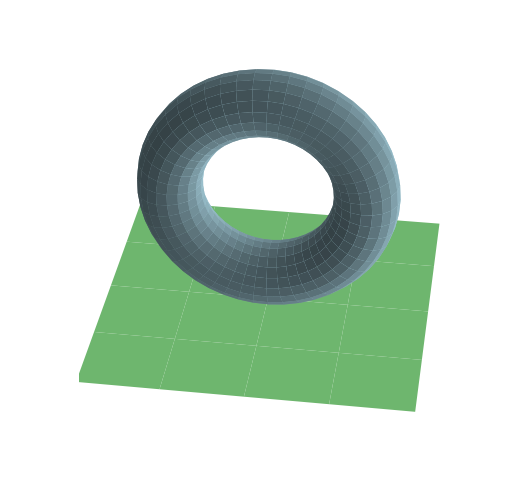
\includegraphics[width=0.6\linewidth]{resources/Me-Diagram1-torus-plane.png}
    \label{fig:me-diagram1}
    \caption{Torus auf der Ebene}
\end{figure}

Es sei $f$ die Abbildung vom Torus nach $\R$, die jedem Punkt den minimalen
Abstand zu der eingezeichneten Ebene zuordnet. 
Die kritischen Punkte dieser Höhenfunktion sind $p$, $q$, $r$ und $s$.
Man stellt sich vor, dass man den Torus nach und nach mit Wasser befüllt. Dann 
ist für $a \in \R$ $M^a = f^{-1}(-\infty, a]$ die Menge der Punkte die bei der
Wasserhöhe $a$ das Wasser berühren. 

\begin{itemize}
    \item Für $a < 0$ ist $M^a = \varnothing$.
    \item Für $0 \leq a < f(p)$ ist $M^a$ homotopieäquivalent zum Punkt.
    \item Für $f(p) \leq a < f(q)$ ist $M^a$ homotopieäquivalent zum Kreis,
        an dem ein "Henkel" befestigt wurde.
    \item Für $f(q) \leq a < f(r)$ ist $M^a$ Homotopieäquivalent zum Zyliner,
        an dem ein "Henkel" befestigt wurde.
    \item Für $f(s) \leq$ ist $M^a$ der Torus selbst.
\end{itemize}

Wir bemerken: 
\begin{itemize}
    \item Gibt es im Intervall $[a, b]$ keine kritischen Werte, so haben alle
        $M^c$ für $c \in [a, b]$ denselben Homotopie-Typ
    \item Gibt es im Intervall $[a, b]$ genau einen kritischen Wert $c$ und ist
        $ \#f^{-1}(p) = 1$, dann hat $M^b$ den Homotopie-Typ von $M^a$ mit einem 
        Henkel angebracht (Was auch immer das bedeutet).
\end{itemize}

Um diese zwei Aussagen zu präzisieren, brauchen wir einige Definitionen:

\begin{definition}[Deformationsretrakt]
    Sei $X$ ein topologischer Raum und $A \subseteq X$ ein Unterraum von $X$.
    Eine stetige Abbildung $r: X \times [0, 1] \rightarrow X$ heißt 
    \textit{Deformationsretraktion} auf $A$, falls gelten:
    \begin{align*}
        & r(\cdot, 0) = \id_X \\
        & r(X, 1) \subseteq A \\
        & r(\cdot, 1)|_A = \id_A \\
    \end{align*}
    $A$ heißt \textit{Deformationsretrakt}, falls eine Deformationsretraktion
    von $X$ auf $A$ existiert.
\end{definition}

Deformationsretrakte haben einige schöne Eigenschaften. Falls $A$ ein
Deformationsretrakt von $X$ ist, so ist die Inklusion $A \rightarrow X$ eine
Homotopieäquivalenz. Da Homotopieäquivalenz transitiv ist, hat ein weiterer
Deformationsretrakt $B$ von $X$ deshalb denselben Homotopietypen wie $A$. \\
Es eine Tatsache, dass zwei Unterräume $A$ und $B$ genau dan denselben 
Homotopietypen haben, wenn sie beide Deformationsretrakte eines gemeinsamen 
Oberraumes sind. Um dies einzusehen benötigt man weitere topologische 
Theorie.

\begin{definition}[Eine $k$-Zelle anbringen]
    Es sei $X$ ein Topologischer Raum. Seien
    \[ e^k = D^k = \{(x_1, ..., x_k) \in \R^k: x_1^2 + ... + x_k^2 \leq 1\} \]
    \[ \varphi: \del e^k \rightarrow X \text{ stetig } \]
    \[ X \cup_{\varphi} e^k = (X \amalg e^k) / \sim, \text{ wobei } \]
    \[ \del e^k \ni x \sim y \in X \Leftrightarrow \varphi(x) = y \]
    Dann heißt $e^k$ $\lambda$-Zelle, $\varphi$ Anheftungsabbildung 
    und $X \cup_{\varphi} e^k$ heißt $X$ mit einer $k$-Zelle 
    angebracht.
\end{definition}

\textbf{ZEICHNUNG 1-Zelle, 2-Zelle}

Ein Paar Beispiele: 
\begin{itemize}
    \item Eine $0$-Zelle in einen nichtleeren Raum anzubringen 
        verändert diesen nicht, und
        \[\varnothing \cup_{\varphi} e^0 = \ast\]
    \item Eine $1$-Zelle lässt uns Zusammenhangskomponenten mit einer "Schnur"
            verbinden, oder ist das Anheften einer "Schlaufe".
    \item Eine $2$-Zelle anzubringen kann sein wie das anbringen einer Blase oder
        das stopfen eines Loches durch eine "Membran".
\end{itemize}

Eine $k$-Zelle kann also zwei Sachen: "Löcher", die von der $k$-ten Homologie
"gemessen" werden zu erschaffen oder "Löcher", die von der $(k-1)$-ten Homologie
"gemessen" werden zu "stopfen". Wenn wir also unsere Mannigfaltigkeit in 
Bezug auf solche Zellen bringen können, dann macht es uns das leichter die 
Topologie (und Homologie) der Mannigfaltigkeit besser zu verstehen. Wenn wir
sogar die gesamte Mannigfaltigkeit durch iteratives anbringen von $k$-Zellen
an den leeren Raum "erschaffen" können, dann können wir einigen Aussagen über 
die Homologie des Raumes machen. 


\begin{theorem}[Erstes Deformationslemma]
    \label{theorem:erstes deformationslemma}
    Es sei $M$ eine glatte Mannigfaltigkeit und $f: M \rightarrow \R$ eine
    glatte Abbildung. Hat $f$ keine kritischen Werte im Intervall [a, b] und ist
    $f^{-1}[a, b]$ kompakt, so existiert ein Diffeomorphismus 
    $M^a \rightarrow M^b$, und $M^a$ ist ein Deformationsretrakt von $M^b$.
\end{theorem}

\begin{theorem}[Zweites Deformations-Lemma]
    \label{theorem:zweites deformationslemma}
    Es sei $M$ eine glatte Mannigfaltigkeit, $f: M \rightarrow \R$ eine glatte
    Abbildung und $p$ ein nicht-degenerierter kritischer Punkt mit Index 
    $k$. Sei $c := f(p)$ und $\varepsilon \geq 0$, sd. 
    $f^{-1}[c - \varepsilon, c + \varepsilon]$ kompakt ist und außer $p$ keine 
    weiteren kritischen Punkte von $f$ beinhaltet. Dann hat $M^{c-\varepsilon}$
    denselben Homotopietypen wie $M^{c - \varepsilon} \cup_{\varphi} e^k$
    für eine Anheftungsabbildung 
    $\varphi: \del e^k \rightarrow M^{c-\varepsilon}$
\end{theorem}


\section{Das erste Deformationslemma}

\begin{definition}[Riemannsche Metrik]
    Eine \textit{Riemannsche Metrik} $g$ ist ein Skalarprodukt 
    \[ g_p:T_pM \times T_pM \to \R \]
    für jeden Punkt $p$, sodass für alle Vektorfelder $X$ und $Y$ die Abbildung 
    $p \to g_p(X(p), Y(p))$ glatt ist.
    Wir schreiben 
    \[ g_p(x, y) = \langle x, y \rangle \]
\end{definition}

\begin{definition}[Gradient]
    Es sei $M$ \textit{Riemannsche Mannigfaltigkeit}, also eine Mannigfaltigkeit
    zusammen mit einer Riemannschen Metrik $g$. Außerdem sei $f: M \to \R$ glatt.
    Dann ist der \textit{Gradient} von $f$ das (einzigartige) 
    Vektorfeld $\grad f$ für das gilt:
    \[ \langle X, \grad f \rangle = \opd fX \]
\end{definition}

Falls $M$ eine Riemannsche Mannigfaltigkeit, $f: M \to \R$ glatt, ist $p \in M$ 
ein kritischer Punkt von $f$ genau dann, wenn $\grad f (p) = 0$. 

Man kann auf jeder Mannigfaltigkeit eine Riemannsche Metrik definieren.

\begin{figure}[H]
    \centering
    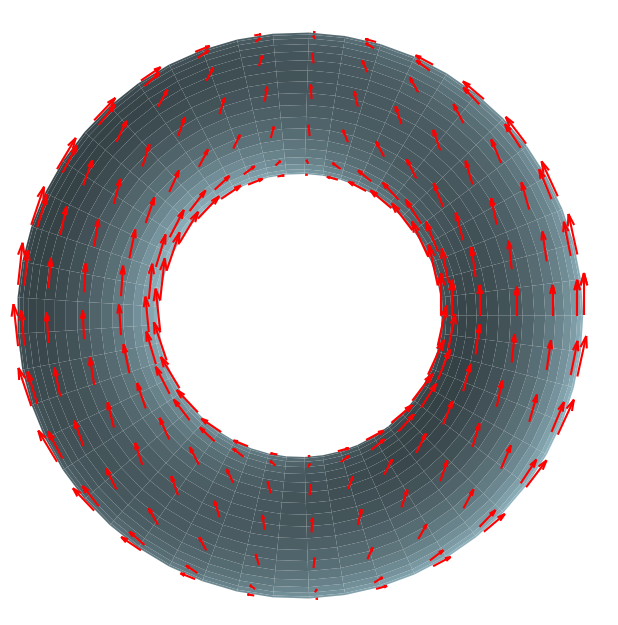
\includegraphics[width=0.7\linewidth]{resources/Me-Diagram4-gradient-of-hightmapping.png}
    \label{fig:me-diagram4}
    \caption{Gradient der Höhenfunktion auf dem Torus}
\end{figure}

\begin{definition}[Flusslinie, Wang]
    Es sei $X$ ein Vektorfeld auf einer glatten Mannigfaltigkeit $M$. Für einen
    glatten Weg $\gamma: I \to M$, $I \subseteq \R$ ein Intervall, 
    definiere für $t_0 \in I$:
    \[ \derive[\gamma]{t}(t_0) = \opd \gamma (t_0) \left(\derive{t}\right) \in T_{\gamma(t_0)}M \]
    wobei $\derive{t} \in T_pM$ das durch die Identität auf $\R$
    induzierte Element im Tangentialraum ist.
    Ein Weg $\gamma: I \to \R$ heißt \textit{Flusslinie} eines Vektorfeldes $X$,
    falls für alle $t_0 \in I$ gilt:
    \[ X(\gamma(t_0)) = \derive[\gamma]{t}(t_0) \]
\end{definition}

\begin{definition}[1-Parameter Gruppe aus Diffeomorphismen]
    Eine \textit{1-Parameter Gruppe aus Diffeomorphismen} ist eine glatte 
    Abbildung
    \[ \varphi: \R \times M \to M \text{, wobei } (t, p) \mapsto \varphi_t(p) \]
    Sodass für alle $s$, $t \in \R$ gilt:
    \[ \varphi_{t + s} = \varphi_t \circ \varphi_s \]
    und 
    \[ \varphi_0 = \id_M \]
    Ich schreibe:
    \[ \varphi_{\bullet}(p): \R \to M ; t \mapsto \varphi_t(p) \]
    Wir sagen eine 1-Parameter Gruppe aus Diffeomorphismen wird von einem
    Vektorfeld $X$ generiert, falls für alle $p \in M$ gilt
    \[ X(p) = \derive[\varphi_{\bullet}(p)]{t}(0) \]
\end{definition}

Ist $\varphi$ eine 1-Parameter Gruppe aus Diffeomorphismern, so ist für alle 
$t \in \R$ $\varphi_t$ ein Diffeomorphismus mit Inverse $\varphi_{-t}$.

Bemerke: Falls $X$ eine 1-Parameter Gruppe aus Diffeomorphismen $\varphi$ erzeugt,
dann ist für alle $p \in M$ der Weg $\varphi_{\bullet}(p)$ eine Flusslinien von $X$, denn
\begin{align*}
    X(\varphi_{t_0}(p)) 
    & = \derive[\varphi_{\bullet}(\varphi_{t_0}(p))]{t}(0)
    = T_0 \varphi_{\bullet}(\varphi_{t_0}(p)) \left(\derive{t}\right) \\
    & = T_0 \varphi_{t_0 + \bullet}(p) \left(\derive{t}\right)
    = T_{t_0} \varphi_{\bullet}(p) \cdot T_0 (t_0 + \id_{\R}) \left(\derive{t}\right) \\
    & = T_{t_0} \varphi_{\bullet}(p) \left(\derive{t}\right)
    = T_{t_0} \varphi_{\bullet}(p) \left(\derive{t}\right) \\
    & = \derive[\varphi_{\bullet}]{t}(t_0)
\end{align*}

\begin{lemma}
    \label{lemma:generierende vektorfelder}
    Es sei $X$ ein Vektorfeld auf einer glatten Mannigfaltigkeit $M$ mit kompaktem 
    Träger. Dann generiert $X$ eine eindeutige 1-Parameter Gruppe aus 
    Diffeomorphismen.
\end{lemma}

\begin{proof} Der Beweis ist recht umfangreich, wird hier aber ausgelassen. \end{proof}

\begin{theorem}[Erstes Deformationslemma]
    \label{theorem:erstes deformationslemma}
    Es sei $M$ eine glatte Mannigfaltigkeit und $f: M \rightarrow \R$ eine
    glatte Abbildung. Hat $f$ keine kritischen Werte im Intervall $[a, b]$ und 
    ist $f^{-1}[a, b]$ kompakt, so existiert ein Diffeomorphismus 
    $M^a \rightarrow M^b$, und $M^a$ ist ein Deformationsretrakt von $M^b$.
\end{theorem}

Das ist genau die erste Aussage, die wir schon am Anfang beim Torus beobachtet 
haben!

Die Idee des Beweises ist es, $M^a$ entlang der Richtung, in die $f$ am stärksten
steigt, also entlang des Gradientenfeldes mit einem Diffeomorphismus $\varphi$ 
"nach oben zu ziehen", bis $\varphi(f^{-1}(a)) = f^{-1}(b)$.

\begin{proof}[Beweis erstes Deformationslemma]
    Es existiert eine kompakte Umgebung $K \in M$ von $f^{-1}[a, b]$. Dies folgt
    aus Whitneys Einbettungssatz und dem Satz von Heine-Borel.
    Sei $\rho: M \to \R$ eine glatte, positive Funktion, sodass
    \[ \rho(p) = 1 / \langle \grad f, \grad f \rangle \]
    für alle $p \in f^{-1}[a, b]$ und die außerhalb von $K$ verschwindet und für
    die für alle $p \in K$, die keine kritischen Punkte sind, gilt: 
    \[ 0 \leq \rho(p) \leq 1 / \langle \grad f, \grad f \rangle \]
    Bemerke dass $\rho$ innerhalb von $f^{-1}[a, b]$ wohldefiniert 
    ist, da sich keine kritischen Punkte im Intervall $[a, b]$ befinden. 
    Definiere ein Vektorfeld $X$ durch
    \[ X(p) = \rho(p) \cdot \grad f (p) \]
    Dann hat $X$ kompakten Träger, erfüllt also die Vorraussetzungen von 
    Lemma~\ref{lemma:generierende vektorfelder}. Sei also $\varphi$ die
    einzigartige 1-Parameter Gruppe aus Diffeomorphismen, die von $X$ generiert
    wird. 
    Wir bekommen für jedes $p \in M$ eine Abbildung 
    $f \circ \varphi_{\bullet}(p): \R \to \R$.
    
    \proofheading{Behauptung 1} Für alle $p \in M$, $t_0 \in \R$ und $q = \varphi_{t_0}(q)$
    ist $\derive{t} f \circ \varphi_{\bullet}(p) (t_0) \in [0, 1]$ und falls $f(\varphi_t(q)) \in [a, b]$
    gilt sogar $\derive{t} f \circ \varphi_{\bullet}(q) (t_0) = 1$.

    Für $q = \varphi_{t_0}(p)$:
    \begin{align*}
        \derive{t} f \circ \varphi_{t_0}(p)
        & = T_{\varphi_{t_0}(p)} f \cdot T_{t_0}\varphi_{\bullet}(p) \left( \derive{t} \right)
        = \opd f (q) \cdot X(q) \\
        & = \langle X(q), \grad f (q) \rangle 
        = \rho(q) \langle \grad f (q), \grad f (q) \rangle \in [0, 1]
    \end{align*}
    
    $f \circ \varphi_{\bullet}(p)$ ist also monoton wachsend für alle $p \in M$.

    Falls sogar $f(\varphi_p(t_0)) \in [a, b]$, dann gilt
    \[ \frac{d}{dt} f \circ \varphi^p (t_0) = 1 \]
    \sectiondone

    \proofheading{Behauptung 2} Für $p \in f^{-1}(a)$, $t_0 \in [0, b-a]$ gilt $f(\varphi_{t_0}(p)) \in [a, b]$.
    
    \[ f(\varphi_{t_0}(p)) \geq f(\varphi_0(p)) = a \]
    und
    \begin{align*}
        f(\varphi_t(p)) 
        & \leq f(\varphi_{b-a}(p)) \\
        & = \int_0^{b-a}\derive{t} f(\varphi_t(p)) \opd t + f(\varphi_0(p)) \\
        & = \int_0^{b-a}\rho(\varphi_t(p)) \langle \grad f (\varphi_t(p)), \grad f (\varphi_t(p)) \rangle \opd t + a \\
        & \leq \int_0^{b-a} 1 \, \opd t + a \\
        & = b
    \end{align*}
    \sectiondone

    \proofheading{Behauptung 3} Unter $\varphi_{b-a}$ wird das Level-Set 
    $f^{-1}(a)$ auf das Level-Set $f^{-1}(b)$ abgebildet.
     
    Für $p \in f^{-1}(a)$ gilt:
    \[ \varphi_{a-a}(p) = \varphi_0(p) = p \]
    und für $t_0 \in [0, b - a]$ gilt wegen Behauptung 1 und 2
    \[ \derive{t}f(\varphi_{\id_{\R} - a}(p)) (t_0) = 1 \]
    also
    \[ f(\varphi_{b - a}(p)) = f(\varphi_{0}(p)) + (b - a) = b \]
    Genauso gilt für $q \in f^{-1}(b)$: $f(\varphi_{a - b}(q)) = a$, also 
    $\varphi_{b - a}(f^{-1}(a)) = f^{-1}(b)$.
    \sectiondone

    \proofheading{Behauptung 4} $\varphi_{b - a} (M^a) = M^b$

    "$\subseteq$": Sei $p \in M^a$. OBdA. existiert $s \in [0, b-a]$, sodass 
    $f(\varphi_s(p)) = a$, ansonsten gilt für alle 
    $s \in [0, b-a]: f(\varphi_s(p)) \leq a < b$. Dann gilt
    \[ f(\varphi_{b-a}(p)) \leq f(\varphi_{b-a+s}(p)) = f(\varphi_{b-a}(\varphi_s(p))) = b \] 
    "$\supseteq$": Analog.
    \sectiondone

    Damit ist $\left. \varphi_{b-a} \right\vert_{M^a}$ ein Diffeomorphismus zwischen
    $M^a$ und $M^b$. 

    Betrachte nun $r: M^b \times \R \to M^b$,
    \[  
        r(p, t) = \begin{cases}
            p & \text{ falls } f(p) \leq a \\
            \varphi_{t(a - f(p))}(p) & \text{ falls } a \leq f(p) \leq b 
        \end{cases}
    \]

    Dann ist $r$ stetig, $r(\cdot, 0)$ ist die Identität auf $M^b$, 
    $r(\cdot, 1)|_{M^a}$ ist die Identität auf $M^a$ und 
    $r(1, M^b) \subseteq M^a$, also ist $M^a$ ein Deformationsretrakt von $M^b$.

\end{proof}

\begin{corollary}
    Es sei $M$ eine Mannigfaltigkeit, $f: M \to \R$ eine glatte Funktion ohne
    kritische Werte in $[a, b]$. dann ist $f^{-1}[a, b]$ diffeomorph zu den
    Mannigfaltigkeiten mit Rand $f^{-1}(a) \times [a, b]$ und 
    $f^{-1}(b) \times [a, b]$.
\end{corollary}


\section{Das zweite Deformationslemma}

\begin{theorem}[Zweites Deformations-Lemma]
    \label{theorem:zweites deformationslemma}
    Es sei $M$ eine glatte Mannigfaltigkeit, $f: M \rightarrow \R$ eine glatte
    Abbildung und $p$ ein nicht-degenerierter kritischer Punkt mit Index 
    $k$. Sei $c := f(p)$ und $\varepsilon \geq 0$, sd. 
    $f^{-1}[c - \varepsilon, c + \varepsilon]$ kompakt ist und außer $p$ keine 
    weiteren kritischen Punkte von $f$ beinhaltet. Dann hat $M^{c-\varepsilon}$
    denselben Homotopietypen wie $M^{c - \varepsilon} \cup e^k$.
\end{theorem}

Das ist die zweite Aussage, die wir am Anfang am Beispiel des Torus beobachtet haben!

Die Idee für den Beweis ist, sich eine neue Funktion $F: M \to \R$ zu definieren,
die Außerhalb von einer kleinen Umgebung von $p$ $f$ entspricht und in der 
Umgebung etwas kleiner ist. Dann bekommen wir die folgende Situation:

\begin{figure}[H]
    \centering
    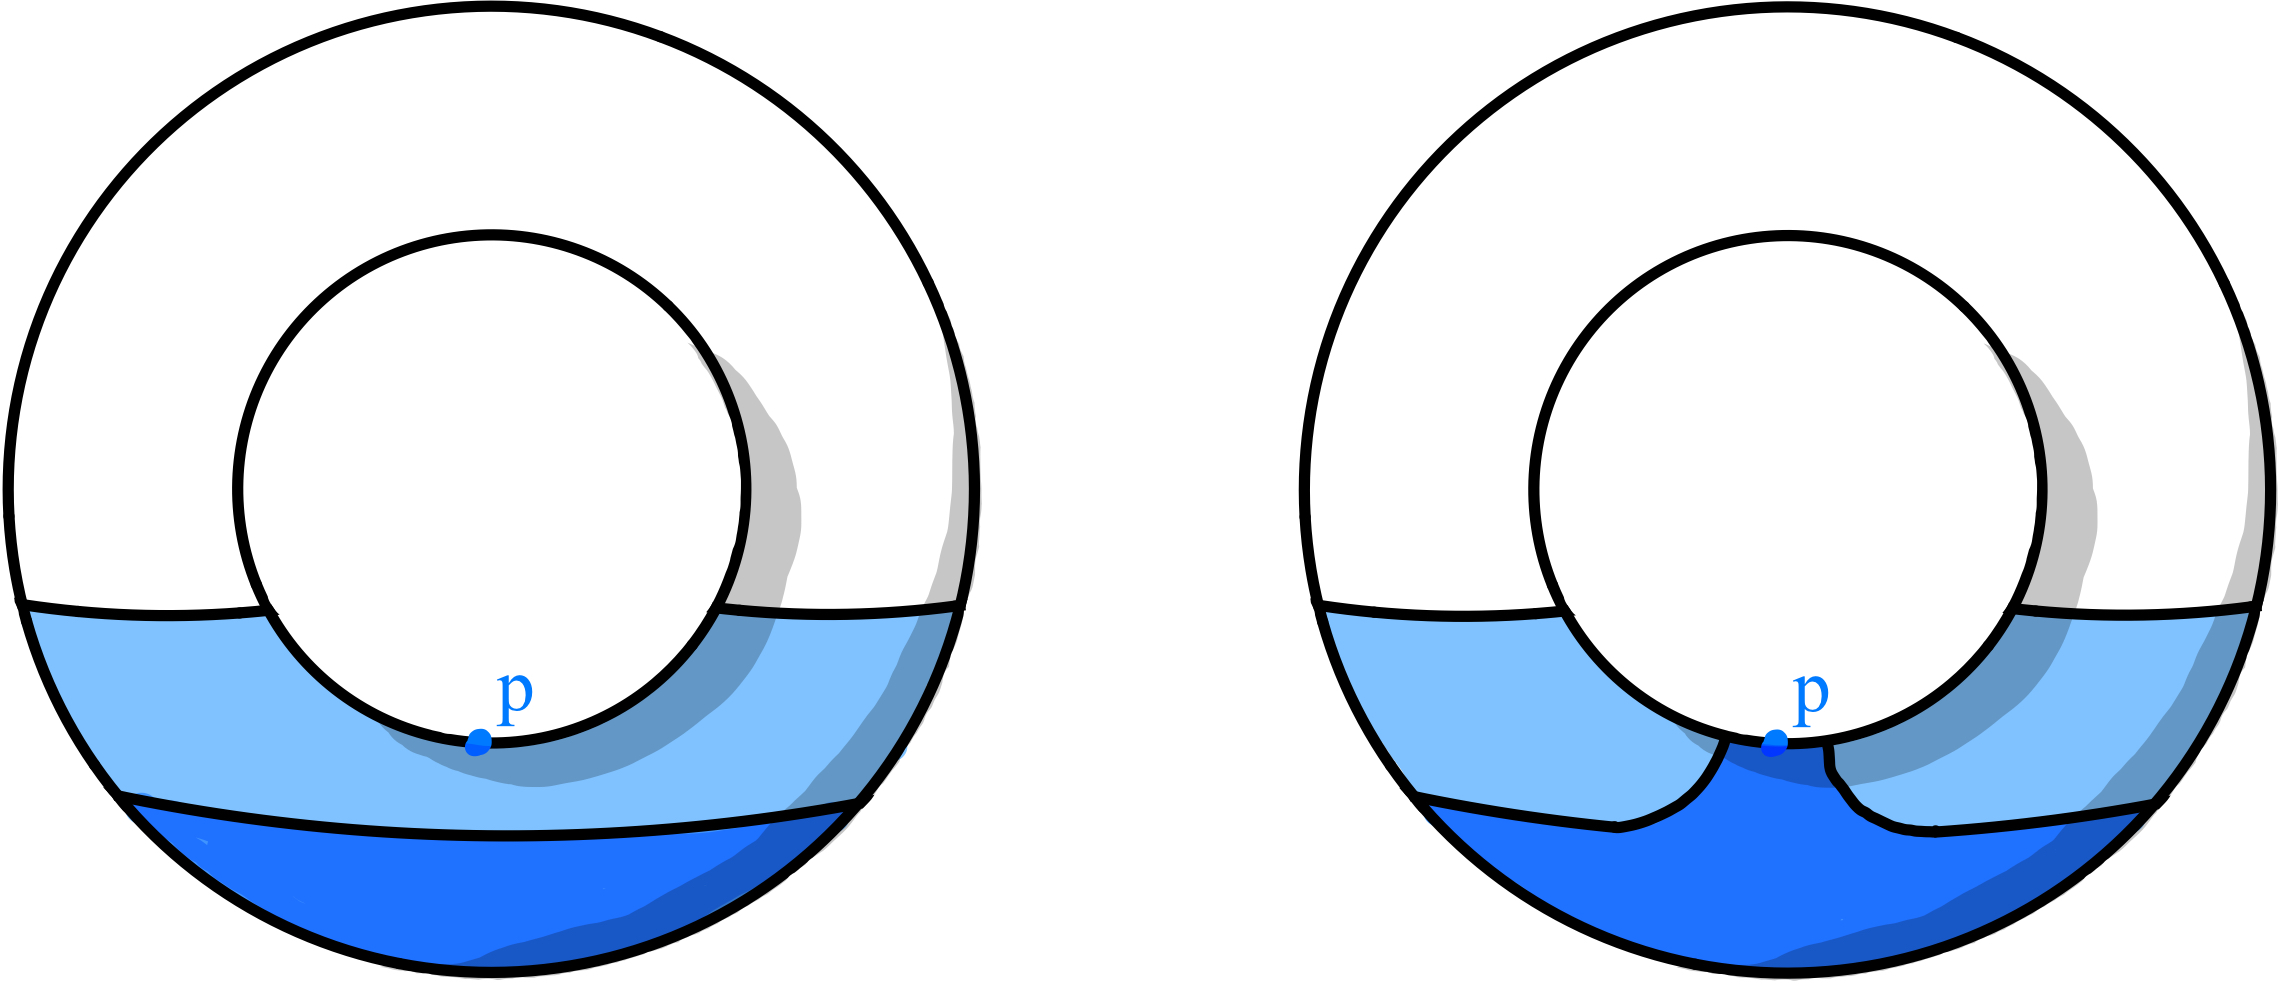
\includegraphics[width=0.8\linewidth]{resources/Me-Diagram5-sublevelsets-of-f-and-F.jpeg}
    \label{fig:me-diagram5}
    \caption{Die Niveaumengen von $f$ (links) und $F$ (rechts)}
\end{figure}

Wir wollen also, dass $M^{c + \varepsilon} = F^{-1}(- \infty, c + \varepsilon]$ 
gilt und $F^{-1}(-\infty, c - \varepsilon]$ fast dasselbe ist wie 
$M^{c - \varepsilon}$, nur dass $F^{-1}(-\infty, c - \varepsilon]$ einen "Henkel"
enthält der den kritischen Punkt $p$ enthält.

\begin{proof}[Beweis zweites Deformationslemma]
    Sei $c := f(p)$. Mit dem Morse-Lemma können wir lokale Koordinaten 
    $\varphi = (u_1, ..., u_n)$ in einer Umgebung $U$ von $p$ wählen, sodass
    \[ f = c - u_1^2 - ... - u_k^2 + u_{k+1}^2 + ... + u_n^2 \]
    in dieser Umgebung, und sodass für den kritischen Punkt $p$ gilt:
    \[ u_1(p) = ... = u_n(p) = 0 \]

    Sei oBdA. $\varepsilon > 0$ klein genug, sodass 
    \begin{enumerate}
        \item $f^{-1}[c - \varepsilon, c + \varepsilon]$ kompakt ist und keine
            kritischen Punkte außer $p$ enthält
        \item $\{ x \in \R^n: \lVert x \rVert^2 \leq 2 \varepsilon \} \subseteq \varphi(U) $
    \end{enumerate}

    Wähle nun die $k$-Zelle 
    \[ 
        e^k := \{ p \in M: (u_1(p))^2 + ... + (u_k(p))^2 \leq \varepsilon 
        \text{ und } u_{k+1}(p) = ... = u_n(p) = 0 \} 
    \]

    Wir bekommen die folgende Situation:

    \begin{figure}[H]
        \centering
        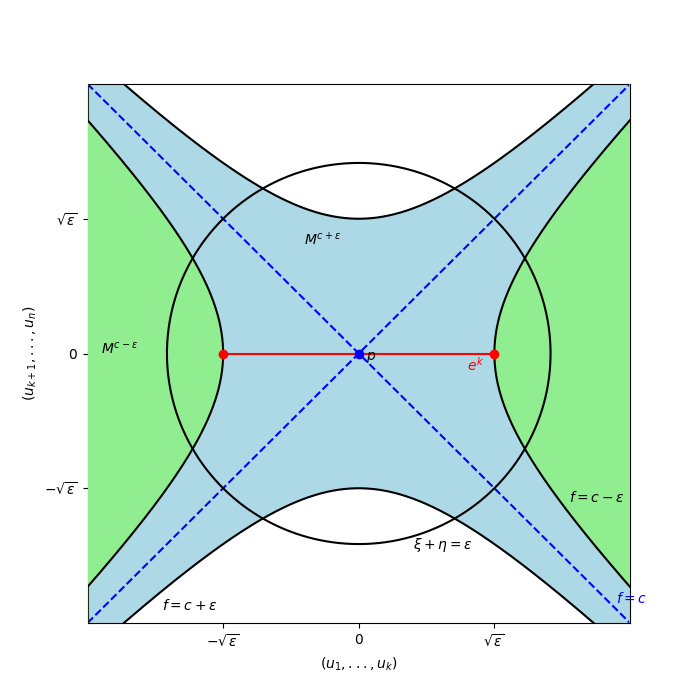
\includegraphics[width=0.8\linewidth]{resources/Me-Diagram6-U-parameterized.png}
        \label{fig:me-diagram6}
        \caption{U parametrisiert}
    \end{figure}

    Nun definiere eine glatte Funktion $\mu: \R \to \R$ mit den Eigenschaften:

    \begin{enumerate}
        \item $ \mu(0) > \varepsilon $
        \item $ \mu(r) = 0 $ falls $ r \geq 2 \varepsilon $
        \item $ -1 < \mu'(r) \leq 0 $ für alle $ r \in \R $
    \end{enumerate}

    Sei nun $F$ außerhalb von $U$ gleich $f$, und sei
    \[ F = f - \mu(u_1^2 + ... + u_k^2 + 2u_{k+1}^2 + ... + 2u_n^2) \]

    $F$ ist wohldefiniert und glatt, da $F$ außerhalb des Kreises mit Radius 
    $\sqrt{2\varepsilon}$ mit $f$ übereinstimmt und der gesamte Kreis in $U$ 
    enthalten ist. Damit haben wir einen guten Kandidaten foür $F$ gefunden.

    Wir definieren nun

    \begin{align*}
        & \eta, \xi: U \to [0, \infty) \\
        & \xi = u_1^2 + ... + u_k^2 \\
        & \eta = u_{k + 1}^2 + ... + e_n^2
    \end{align*}

    Dann gilt innerhalb von $U$:
    \[ f = c - \xi + \eta \]
    und 
    \[ F = f - \mu(\xi + 2 \eta) = c - \xi + \eta - \mu(\xi + 2 \eta) \]

    Jetzt wollen wir überprüfen:
    \begin{enumerate}
        \item $F^{-1}(-\infty, c + \varepsilon] = M^{c + \varepsilon}$.
        \item $F^{-1}(-\infty, c - \varepsilon]$ ist ein Deformationsretrakt von 
            $M^{c + \varepsilon}$.
        \item $M^{c - \varepsilon} \cup e^k$ ist ein Deformationsretrakt von
            $F^{-1}(-\infty, c - \varepsilon]$.
    \end{enumerate}

    Dann folgt schon die Behauptung.

    \proofheading{Behauptung 1} $F^{-1}(-\infty, c + \varepsilon] = M^{c + \varepsilon}$

    Sei $q \in M$. Falls gilt $\xi(q) + 2 \eta(q) > 2 \varepsilon$ gilt 
    $F(q) = f(q) - \mu(\xi(q) + 2\eta(q)) = f(q)$,
    also gelte oBdA.
    \[ \xi(q) + 2 \eta(q) \leq 2 \varepsilon \]
    Dann:
    \[ F(q) \leq f(q) = c - \xi(q) + \eta(q) \leq c + \frac{1}{2}\xi(q) + \eta(q) \leq c + \varepsilon \]
    \sectiondone

    \proofheading{Behauptung 2} $F^{-1}(-\infty, c - \varepsilon]$ ist ein
    Deformationsretrakt von $M^{c + \varepsilon}$.

    Bemerke: Die kritischen Punkte von $F$ stimmen mit denen von $f$ überein, 
    denn:

    \[ \pderive[F]{\xi} = -1 - \mu'(\xi + 2\eta)  < 0 \]
    und
    \[ \pderive[F]{\eta} = 1 - 2 \mu'(\xi + 2\eta) \geq 1 \]
    Insbsondere sind diese beiden Ableitungen also niemals $0$. Da 
    \[ \opd F = \pderive[F]{\xi}\opd \xi + \pderive[F]{\eta} \opd \eta \]
    und $\opd \xi$ und $\opd \eta$ nur in $p$ gleichzeitig Null sind, haben $f$ 
    und $F$  dieselben kritischen Punkte.

    Betrachte die Region $F^{-1}[c - \varepsilon, c + \varepsilon]$. Wegen 
    Behauptung 1 und der Tatsache, dass $F \leq f$ gilt:
    \[ F^{-1}[c - \varepsilon, c + \varepsilon] \subseteq f^{-1}[c - \varepsilon, c + \varepsilon] \]
    Da $f^{-1}[c - \varepsilon, c + \varepsilon]$ kompakt ist und 
    $F^{-1}[c - \varepsilon, c + \varepsilon]$ abgeschlossen ist, ist 
    $F^{-1}[c - \varepsilon, c + \varepsilon]$ auch kompakt. Da $f$ und $F$
    dieselben kritischen Punkte haben kann diese Menge maximal den kritischen 
    Punkt $p$ enthalten, aber
    \[ F(p) = c - \xi(p) + \eta(p) + \mu(\xi(p) + 2\eta(p)) = c - \mu(0) < c - \varepsilon \]
    Also gibt es in $F^{-1}[c - \varepsilon, c + \varepsilon]$ keine kritischen
    Punkte. Mit dem ersten Deformationslemma gilt dann:
    $F^{-1}(- \infty, c - \varepsilon]$ ist Def. Retrakt von 
    $F^{-1}(-\infty, c + \varepsilon] = M^{c + \varepsilon}$.
    \sectiondone

    \proofheading{Behauptung 3} $M^{c - \varepsilon} \cup e^{k}$ ist ein 
    Deformationsretrakt von $F^{-1}(-\infty, c - \varepsilon]$.

    Diese Aussage ergibt nur Sinn, falls 
    $M^{c - \varepsilon} \cup e^{k} \subseteq F^(-\infty, c - \varepsilon]$.
    Wir wissen schon, dass $M^{c - \varepsilon} \subseteq F^{-1}(c - \varepsilon]$.

    Sei $q \in e^k$, dann gilt $\xi(p) = 0 \leq \xi(q) \leq 1$. Da 
    $\pderive[F]{\xi} < 0$, gilt dann
    \[ F(q) \leq F(p) < c - \varepsilon \]

    Also ergibt sich folgende Situation:

    \begin{figure}[H]
        \centering
        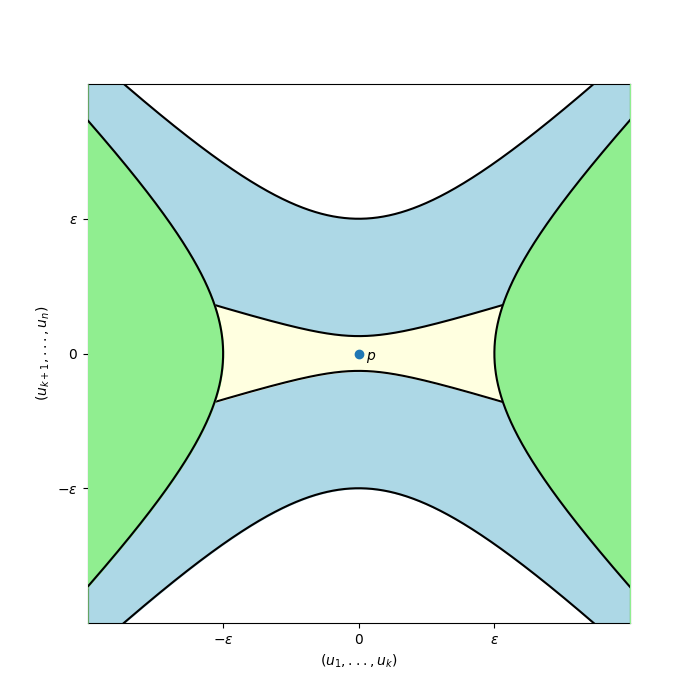
\includegraphics[width=0.8\linewidth]{resources/Me-Diagram7-handle.png}
        \label{fig:me-diagram7}
        \caption{Henkel}
    \end{figure}

    Die hellgrün eingefärbte Fläche ist $M^{c - \varepsilon}$ die hellgelbe
    zusammen mit der hellgrünen Fläch ist $F^{-1}(-\infty, c - \varepsilon]$. 

    Dafür konstruieren wir eine Deformationsretraktion
    $r: F^{-1}(-\infty, c - \varepsilon] \times [0,1] \to F^{-1}(-\infty, c - \varepsilon]$
    für $q \in F^{-1}(-\infty, c - \varepsilon], t \in [0, 1]$, die 
    $F^{-1}(-\infty, c - \varepsilon] - M^{c - \varepsilon}$ auf $e^k$ 
    deformiert, wie folgt.

    \[
        r(q, t) = \begin{cases}
            \varphi^{-1} \circ (u_1, ..., u_k, tu_{k + 1}, ..., tu_n)(q)
                & \text{ im Fall 1: } \xi(q) \leq \varepsilon \\
            \varphi^{-1} \circ (u_1, ..., u_k, s_tu_{k + 1}, ..., s_tu_n)(q)
                & \text{ im Fall 2: } \varepsilon \leq \xi(q) \leq \eta(q) + \varepsilon \\
            q & \text{ im Fall 3: } \eta(q) + \varepsilon \leq \xi(q)
        \end{cases}
    \]

    Wobei 

    \[ s_t = t + (1 -t)((\xi - \varepsilon)/\eta)^{1/2} \]

    Die Fälle sind dann wie folgt:

    \begin{figure}[H]
        \centering
        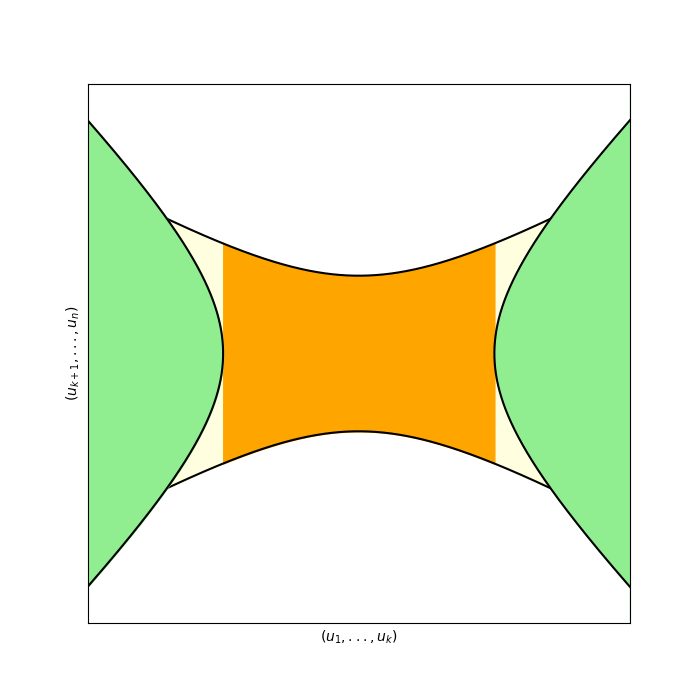
\includegraphics[width=0.8\linewidth]{resources/Me-Diagram9-handle-cases.png}
        \label{me-diagram9}
        \caption{
            Fall 3 ist $M^{c - \varepsilon}$, also die grün eingefärbte Fläche, die
            orangene Fläche ist Fall 1 und die gelbe ist Fall 2.
        }
    \end{figure}

    Wir müssen überprüfen:
    \begin{enumerate}
        \item $r$ ist wohldefiniert und stetig
        \item $r(F^{-1}(-\infty, c - \varepsilon], 0) \subseteq M^{c - \varepsilon} \cup e^k$
        \item $r(\cdot, 1) = \id_{F^{-1}(-\infty, c - \varepsilon]}$ und 
            $\left. r(\cdot , 0) \right\vert_{M^{c - \varepsilon} \cup e^k} 
            = \id_{M^{c - \varepsilon} \cup e^k}$
    \end{enumerate}

    3. ist einfach nachzurechnen. In Fall 1 und Fall 3 ist 2. offensichtlich
    wahr. Für Fall 2 gilt:
    \begin{align*} 
        f(r(0, q)) & = 
            f\left( \varphi^{-1} \left(u_1(q), ..., u_k(q), 
            \left( \frac{\xi(q) - \varepsilon}{\eta(q)} \right)^{1/2}u_{k + 1}(q), ...,
            \left( \frac{\xi(q) - \varepsilon}{\eta(q)} \right)^{1/2}u_n(q)
            \right)
            \right) \\
        & = c - \xi(q)
            + \left( \left( \frac{\xi(q) - \varepsilon}{\eta(q)} \right)^{1/2}u_{k + 1}(q) \right)^2 + ... 
            + \left( \left( \frac{\xi(q) - \varepsilon}{\eta(q)} \right)^{1/2}u_n(q) \right)^2 \\
        & = c - \left( \frac{\xi(q) - \varepsilon}{\eta(q)} \right) \eta(q) \\
        & = c - \varepsilon
    \end{align*}
    also ist $r(0, q) \in f^{-1}(c - \varepsilon)$. Um 1. zu prüfen müssen wir 
    Stetigkeit in den Grenzfällen überprüfen:
    \begin{align*}
        & \text{For } \xi(q) = \varepsilon \text{ : }
            & s_t(q)  =t + (1 - t)((\varepsilon - \varepsilon)/\eta(q))^{1/2} = t \\
        & \text{For } \eta(q) + \varepsilon = \xi(q) \text{ : }
            & s_t(q) = t + (1 - t)((\xi(q) - \varepsilon)/(\xi(q) - \varepsilon))^{1/2} = 1
    \end{align*}

    Das einzig andere Problem was wir bekommen könnten ist nun in Fall 2 falls
    $\eta \to 0$. In Fall 1 und Fall 3 bekommen wir für $q$ mit $\eta(q) = 0$:
    $r(q, t) = \varphi^{-1} \circ (u_1, ..., u_k, 0, ..., 0)(q)$, also wollen
    wir zeigen dass für $\eta \in $ Fall 2 mit $\eta \to 0$ gilt $s_tu_i \to 0$
    für $i \in \{k+1, ..., n\}$. In Fall 2 gilt
    $0 \leq \xi - \varepsilon \leq \eta$. Dann gilt:

    \begin{align*}
        \lim\limits_{\eta \to 0} | s_t u_i |
           & = \lim\limits_{\eta \to 0} (1 - t)((\xi - \varepsilon)/\eta)^{1/2} | u_i | \\
           & \leq \lim\limits_{\eta \to 0} (1 - t)(\eta/\eta)^{1/2}|u_i| \\
           & = \lim\limits_{\eta \to 0} (1 - t)|u_i| = 0 
    \end{align*}
    
    Also ist $r$ stetig.
    \sectiondone

    Mit Behauptung 3 und 4 bekommen wir
    \[ M^{c + \varepsilon} \simeq F^{-1}(c - \varepsilon] \]
    und 
    \[ F^{-1}(-\infty, c - \varepsilon] \simeq M^{c - \varepsilon} \cup e^k \]
    Also folgt die Behauptung:
    \[ M^{c + \varepsilon} \simeq M^{c - \varepsilon} \cup e^k \]

\end{proof}

\begin{corollary}
    Allgemeiner gilt sogar: Angenommen es gibt $m$ kritische Punkte 
    $p_1, ..., p_m$ mit Indizes $k_1, ..., k_m$ in $f^{-1}(c)$. Dann gilt
    \[ M^{c + \varepsilon} \simeq M^{c - \varepsilon} \cup e^{k_1} \cup ... \cup e^{k_m} \]

    Die Anheftungssabbildungen können hier so gewählt werden, dass ihre Bilder 
    disjunkt in $M^{c + \varepsilon}$ liegen, also funktioniert hier unsere 
    ursprüngliche Definition vom Anheften einer $k$-Zelle noch immer.
\end{corollary}


\section{Anwendungen}

\begin{theorem}
    \label{theorem:Sn}
    Sei $M$ eine $n$-dimensionale Mannigfaltigkeit, sodass eine glatte Funktion
    $f: M \to \R$ existiert, die genau zwei kritische Punkte besitzt, die beide
    nicht degeneriert sind. Dann ist $M$ homeomorph zu $S^n$.
\end{theorem}

\begin{proof}
    Seien $p$ und $q$ die kritischen Werte mit $f(p) = a < b = f(q)$. Mit dem 
    Morse Lemma existiert dann $\varepsilon > 0$, sodass 
    $f^{-1}[a, a + \varepsilon]$ und $f^{-1}[b - \varepsilon, b]$ diffeomorph
    zu einer $n$-Zelle $e^n$ sind. 
    Mit dem ersten Deformationslemma~\ref{theorem:erstes deformationslemma} ist
    $f^{-1}[a - \varepsilon, b - \varepsilon]$ deffeomorph zu 
    $\del e^n \times [0, 1]$. Dann ist $M$ der Zylinder $\del e^n \times [0, 1]$ 
    mit $e^n$ an beiden seiten des Zylinders angebracht. Sei 
    $\operatorname{pr}_1: S^n \to \R$ die Projektion auf die erste Koodinate von
    $S^n \subset \R^{n + 1}$. Dann hat $\operatorname{pr}_1$ genau zwei kritische 
    Punkte, beide sind nicht degeneriert, also gilt $M \cong S^n$.
\end{proof}

\begin{theorem}
    \label{theorem:CW-komplex}
    Sei $M$ eine Mannigfaltigkeit und $f: M \to \R$ eine glatte Funktion mit 
    ausschließlich nicht degenerierten kritischen Punkten $p_1, ..., p_m$. 
    Dann besitzt $M$ den Homotopie-Typen von einem CW-Komplex mit einer $k$-Zelle 
    für jeden kritischen Punkt mit Index $k$.
\end{theorem}

\begin{proof}
    Der Beweis ist recht involviert, aber im wesentlichen folgt die Aussage aus
    dem zweiten Deformationslemma~\ref{theorem:zweites deformationslemma}.
\end{proof}

\begin{theorem}[Morse Ungleichungen]
    Sei $M$ eine kompakte Mannigfaltigkeit, $f: M \to \R$ eine glatte Funktion
    mit ausschließlich nicht degenerierten kritischen Punkten. Sei $C_k$ die
    Anzahl der kritischen Punkte mit Index $k$. Sei $\betti_k(M)$ die $k$-te 
    Betti-Zahl von $M$ und $\chi(M)$ die Euler-Charakteristik von $M$. 
    Dann gelten:
    \begin{enumerate}
        \item $ \betti_k(M) \leq C_k $ 
        \item $ \chi(M) = \sum_k (-1)^k \cdot C_k $
        \item $ \betti_k(M) - b_{k - 1}(M) + ... \pm \betti_0(M) 
            \leq C_k - C_{k-1} + ... \pm C_0 $
    \end{enumerate}
\end{theorem}

\begin{proof}
    Auch hierfolgt die Behauptung wesentlich aus dem zweiten 
    Deformationslemma~\ref{theorem:zweites deformationslemma}:
    Wir definieren $\betti_k$ und $\chi$ für ein Raumpaar $(X, Y)$:
    \[ \betti_k(X, Y) = \dim (\Hom_k (X, Y)) \]
    und 
    \[ \chi(X, Y) = \sum_k (-1)^k \betti_k(X, Y) \]
    Man kann zeigen, dass $\betti_k$ subadditiv und $\chi$ addutiv sind, also
    dass für $Z \subseteq Y \subseteq X$ gilt
    \[ \betti_k(X, Z) \leq \betti_k(X, Y) + \betti_k(Y, Z) \]
    und 
    \[ \chi(X, Z) = \chi(X, Y) + \chi(Y, Z) \]
    Außerdem zeigt man, dass für $X_0 \subseteq ... \subseteq X_n$ gilt
    \[ S(X_n, X_0) \leq \sum_i S(X_i, X_{i-1}) \]
    falls $S$ subadditiv, und dass falls $S$ additiv ist sogar Gleichheit gilt.
    
    ObdA hat $f$ nur isolierte kritische Punkte. Seien dann 
    $a_0, ..., a_m \in \R$ so gewählt, dass $M^{a_i}$ genau $i$ kritische Punkte
    enthalten und $M^{a_m} = M$. Dann gilt schon $M^0 = \varnothing$. Sei nun $k_i$
    der Index des kritischen Punktes in $M^{a_i} - M^{a_{i-1}}$. Dann gilt:
    \begin{align*}
        \Hom_k(M^{a_i}, M^{a_{i-1}}) 
            & = \Hom_k(M^{a_{i-1}} \cup e^{k_i}, M^{a_{i-1}})
            & \text{ (wegen des zweiten Deformationslemmas) } \\
        & = \Hom_k(e^{k_i}, \del e^{k_i})
            & \text{ (wegen der Ausschneidungseigenschaft) } \\
        & = \Hom_k(S^{k_i}, \ast)
    \end{align*}

    Also haben wir
    \[ 
        H_k(M^{a_i}, M^{a_{i-1}}) = \begin{cases}
            \R &\text{ falls } k = k_i \\
            0 & \text{ sonst }
        \end{cases}
    \]
    Da $\betti_k$ subadditiv ist gilt 
    \begin{align*}
        \betti_k(M) 
           & \leq \sum_i \betti_k(M^{a_i}, M^{a_{i-1}}) \\
           & = \sum_i \dim(\Hom_k(M^{a_i}, M^{a_{i-1}})) \\
           & = C_k
    \end{align*}
    
    Und da $\chi$ additiv ist gilt
    \begin{align*}
        \chi(M) 
           & = \sum_i \chi (M^{a_i}, M^{a_{i-1}}) \\
           & = \sum_i \sum_k (-1)^k \dim \Hom_k (M^{a_i}, M^{a_{i-1}}) \\
           & = \sum_k (-1)^k C_k
    \end{align*}

    3. folgt aus der Tatsache, dass $S_k$ subadditiv ist, wobei 
    \[ 
      S_k(X, Y) 
      = \betti_k(X, Y) - \betti_{k - 1}(X, Y) + ... \pm \betti_{0} 
    \]

    Dann gilt wieder
    \begin{align*} 
        S_k (M) 
            & \leq \sum_{i = 1}^m (-1)^i S_k(M^{a_i}, M^{a_{i-1}}) \\
            & = \sum_{i = 1}^m \betti_k(M^{a_i}, M^{a_{i-1}}) 
            - \betti_{k - 1}(M^{a_i}, M^{a_{i-1}})
            + ... \pm \betti_0(M^{a_i}, M^{a_{i-1}})
    \end{align*}
    aber gerade haben wir schon gesehen, dass gilt
    \[ 
        \betti_k(M^{a_i}, M^{a^{i-1}}) = 
            \begin{cases}
                1 & \text{ if } k = i \\
                0 & \text{ else }
            \end{cases}
    \]
    Also gilt
    \[ 
        \sum_{i = 1}^m \betti_k(M^{a_i}, M^{a_{i-1}}) 
            - \betti_{k - 1}(M^{a_i}, M^{a_{i-1}})
            + ... \pm \betti_0(M^{a_i}, M^{a_{i-1}})
        = C_k - C_{k - 1} + ... \pm C_0
    \]

\end{proof}


\end{document}
